%!TEX root = ../thesis.tex
%*******************************************************************************
%*********************************** First Chapter *****************************
%*******************************************************************************

\chapter{Herramientas BPM (Business Process Management) y Detección de Fallas}  %Title of the First Chapter

\ifpdf
    \graphicspath{{Chapter1/Figs/Raster/}{Chapter1/Figs/PDF/}{Chapter1/Figs/}}
\else
    \graphicspath{{Chapter1/Figs/Vector/}{Chapter1/Figs/}}
\fi

Al masificarse el uso de los sistemas de cómputo en las empresas y con el surgimiento de la comunicación digital, las organizaciones cambiaron drásticamente la manera de operar sus procesos de negocio, dado que con este nuevo desarrollo tecnológico fue posible automatizar gran parte de dichos procesos. Las primeras herramientas desarrolladas para la automaticación de procesos de negocio fueron los denominados sistemas WfM (Workflow Management Systems), los cuales aún se encuentran vigentes, sin embargo, estos sistemas no permiten controlar los procesos de negocio eficientemente. Dado lo anterior, surgieron los sistemas BPM (Business Process Management Systems), los cuales no solo permiten automatizar la ejecución de los procesos de negocio, si no que también se enfocan en la gestión de las operaciones, la organización del trabajo, y buscan que los procesos de negocio sean más eficientes [55, 56]. Otra de las funcionalidades más importantes de los sistemas WfM/BPM a parte de permitir automatizar en gran medida los procesos de negocio, es que permiten modelar los procesos de negocio a partir de la definición de flujos de trabajo o workflows [1], con lo cual es posible abstraer los procesos de negocio más fácilmente, permitiendo que su implementación sea más rápida. 

Aunque constantemente estas herramientas BPM han estado evolucionado, aún presentan algunas debilidades al momento de identificar y controlar las excepciones generadas en la operación de los procesos de negocio. 

%********************************** %First Section  **************************************
\section{Gestión de Procesos de Negocio} %Section - 1.1 
\label{section1.1}

La gestión de procesos de negocio (BPM, Business Process Management) es una metodología que busca controlar, analizar y mejorar los procesos de negocio de las organizaciones mediante técnicas, métodos y herramientas de software. Estas últimas denominadas sistemas BPM o en inglés BPM systems. 

La metodología BPM propone un proceso cíclico que permite realizar la implementación de los procesos de negocio organizacionales, permitiendo mejorar continuamente los procesos de negocio. Este ciclo de vida comprende cuatro fases; la fase de diseño del proceso (Process Desing), la de configuración del sistema (System Configuration), la de promulgación del proceso (Process Enactment) y la de diagnóstico (Diagnosis) [1].

La fase de diseño del proceso consiste en realizar un análisis inicial del proceso de negocio a intervenir, y a partir de este análisis realizar todas las definiciones correspondientes para la implementación del proceso. Sin embargo, debido a que los procesos de negocio varían constantemente a lo largo del tiempo, esta fase también consiste en rediseñar un proceso ya existente. Este rediseño no necesariamente involucra una nueva configuración en el sistema, por ejemplo, podría tratarse simplemente de modificar la manera como los usuarios realizan la gestión de los proceso de negocio. 

Luego de realizar todo el análisis de diseño o rediseño del proceso, se continúa con la fase de configuración del sistema, la cual consiste en aplicar todas las parametrizaciones identificadas y definidas en la fase anterior sobre la herramienta BPM. Vale la pena resaltar que estas herramientas generalmente están construidas de tal manera que no sea necesario implementar nuevo código, sin embargo pueden existir excepciones.

La fase de promulgación del proceso consiste en desplegar de manera productiva todas las configuraciones realizadas en la fase anterior. 

Finalmente el proceso termina con la fase de diagnostico, en la cual se analizan los cambios presentados a lo largo dele tiempo, al igual que se identifican los aspectos de mejora que pueden ser aplicados en el proceso de negocio, de tal manera que el ciclo inicie nuevamente con la fase de rediseño del proceso. La figura \ref{fig:CicloVida} ilustra el proceso.

\begin{figure}[htbp!] 
\centering    
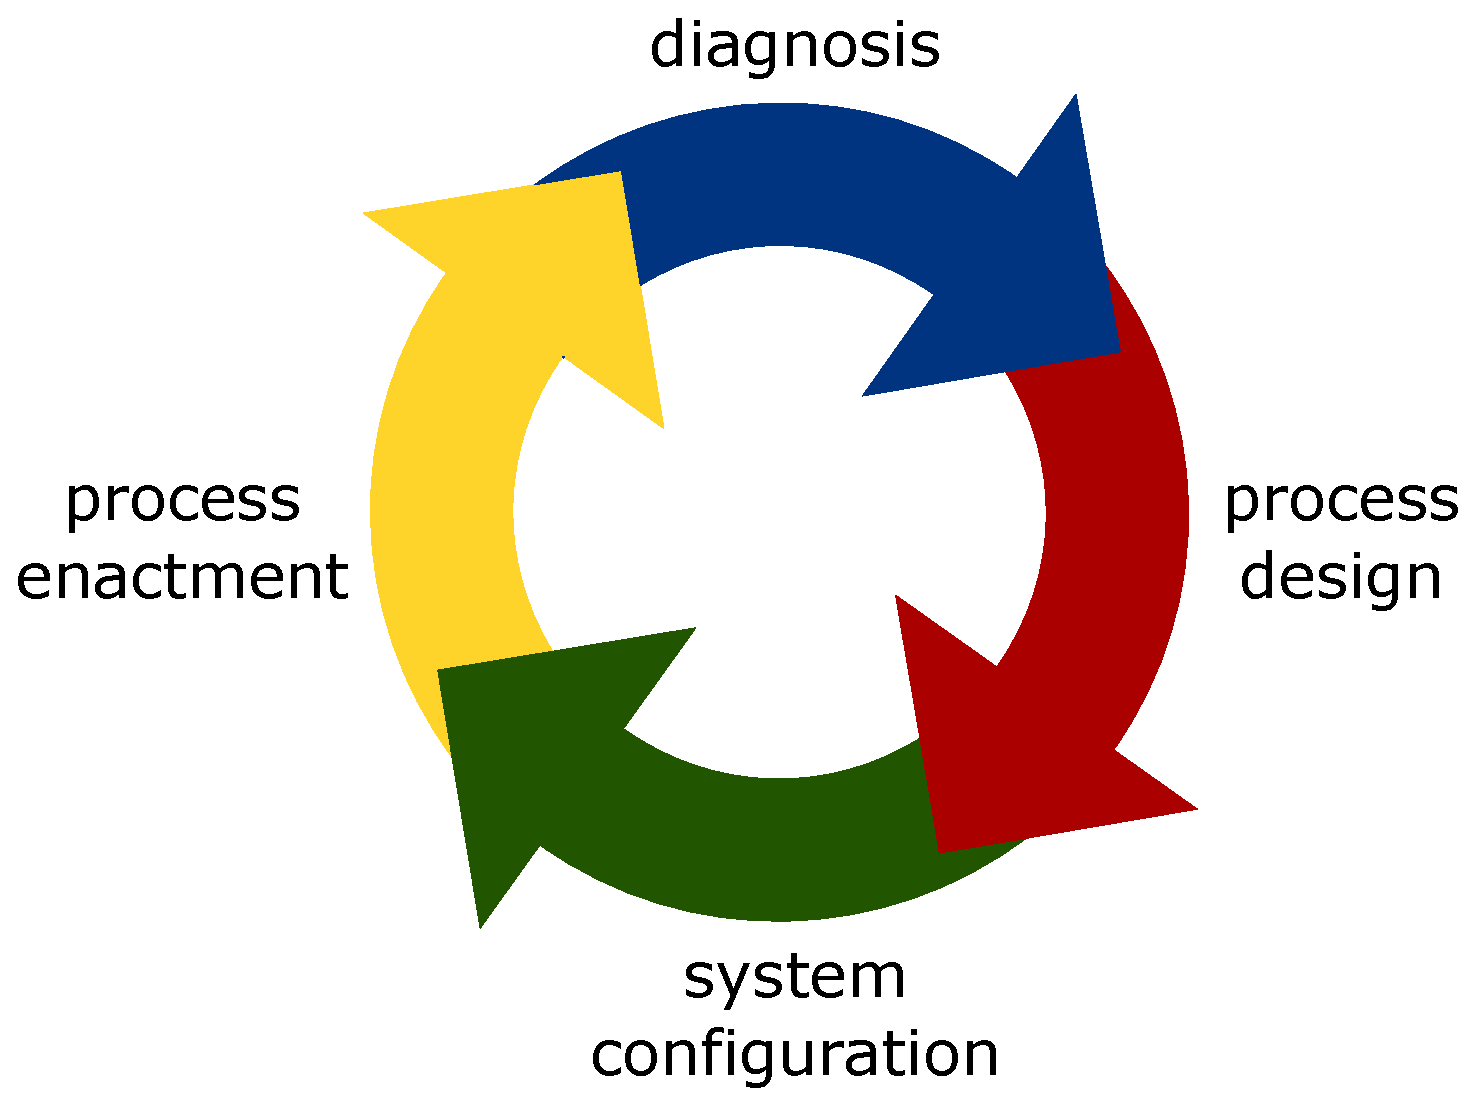
\includegraphics[width=0.5\textwidth]{Chapter1/Figs/Figure_lifecycle}
\caption[CicloVida]{Ciclo de vida del proceso de BPM Tomada de [1]}
\label{fig:CicloVida}
\end{figure}

%********************************** %Second Section  **************************************
\section{Sistemas BPM} %Section - 1.2
\label{section1.2}

Antes del surgimiento de los sistemas BPM existían los sistemas WfM, los cuales se enfocan específicamente en automatizar los procesos de negocios, dejando de lado aspectos relacionados con el control y mejoramiento de los procesos. Es por esto que los sistemas BPM tomaron relevancia, pues además de automatizar los procesos de negocios, también se enfocan en la gestión de las operaciones, la organización del trabajo, y buscan que los procesos de negocio sean más eficientes [55, 56]. Adicionalmente, tanto los sistemas BPM como los WfM, permiten obtener múltiples abstracciones de los procesos de negocio mediante la definición de flujos de trabajo o workflows \cite{VanderAalst2004}. En estos flujos de trabajo se define la secuencia de pasos a seguir en la gestión del proceso de negocio, también se definen las decisiones que se deben tomar dentro del proceso a partir de la información dada. Cada instancia de estos flujos de trabajo se denomina un ítem de trabajo o workitem, y se encarga de ejecutar la secuencia de pasos definida en la herramienta BPM teniendo en cuenta información específica. 

Es usual que para cada uno de los ítem de trabajo mencionados anteriormente se registre información relacionada con los sucesos de eventos (event logs), estos hacen referencia a eventos ocurridos dentro del proceso de ejecución de los workitems, y pueden ser almacenados de diferentes maneras, por ejemplo, en una base de datos relacional o en archivos planos. 

Dado que los procesos de negocio constantemente tienen un gran número de procesos activos, las herramientas BPM deben almacenar grandes volúmenes de información relacionada con los sucesos de eventos, al igual que deben manejar adecuadamente la concurrencia, pues es típico que en los procesos de negocio se tengan decenas de miles de elementos de trabajos activos.

Pensando en lo anterior, los sistemas WfM/BPM deben considerar ciertos aspecto importantes, no solamente los relacionados con la concurrencia, si no también los relacionados con la seguridad de la información, la seguridad del sistema, los tiempos de respuesta, la tolerancia a fallas, entre otros. De tal manera que sea posible contar con sistemas robustos y escalables, y que permitan soportar los procesos críticos de las organizaciones. Es por esto que existen algunas propuestas a nivel de arquitectura que buscan garantizar la estabilidad y robustez de las herramientas WfM/BPM [55]. 

En la actualidad existe una institución que se encarga de describir como deben funcionar los sistemas WfM/BPM, al igual de como deben ser construidos, esta entidad se llama Workflow Management Coalition (WfMC), y fue fundada en 1993 [55]. Esta institución propone un esquema de arquitectura para las herramientas BPM o WfM, de tal manera que sea posible contar con un estándar de referencia para el desarrollo y uso de estos sistemas. Algunos de los componentes más relevantes son los siguientes: 

\begin{itemize}
    \item Workflow enactment service, el cual proporciona un entorno de tiempo de ejecución que se encarga del control y la ejecución de los flujos de trabajo. Este es el componente principal de la arquitectura propuesta por el WfMC,  y puede disponer de uno o varios workflow engines, los cuales manejan partes especificas del flujo de trabajo y de los recursos del sistema [55]. 
    
    \item Process definition tools o herramientas de definición de procesos, estas herramientas permiten realizar el diseño de los procesos de negocio por medio de notación de modelado de proceso. También permiten realizar análisis y simulaciones de los procesos de negocio definidos en los flujos de trabajo [55]. 
    
    \item Workflow client applications, este componente permite a los usuarios finales comunicarse con los workflows systems, generalmente mediante el uso de los denominados in-baskets, los cuales presentan los workitems al usuario final de manera ordenada, y sobre los cuales es posible ejecutar tareas específicas.
    
    \item Administration and monitoring tools, estas herramientas de administración y monitoreo buscan controlar todo el proceso, registrando información detallada de los casos.
    
\end{itemize}

\begin{figure}[htbp!] 
\centering    
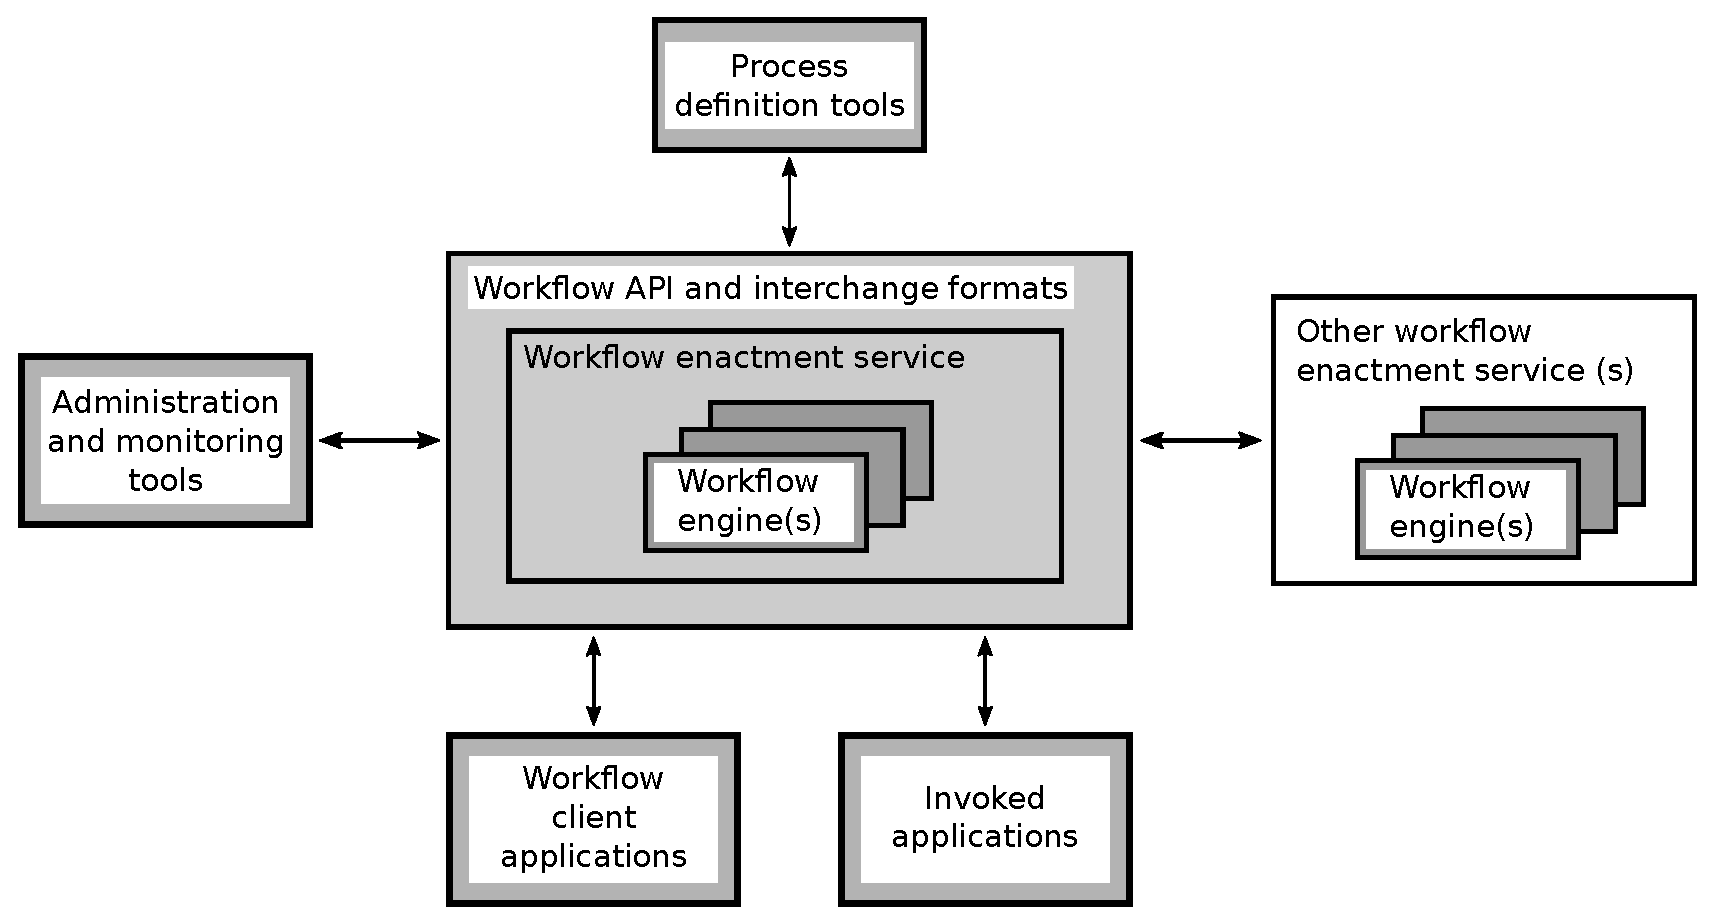
\includegraphics[width=1.0\textwidth]{Chapter1/Figs/Figure_referenceWfMC}
\caption[ReferenceWfMC]{Referencia arquitectura Tomada de [1]}
\label{fig:ReferenceWfMC}
\end{figure}

Los componentes mencionados anteriormente pueden visualizarse en las figuras [55] y (Figura 21 [55]) referencia [1], en esta última también se muestran los componentes de datos usados en los sistemas BPM, al igual que su interacción con los demás componentes.

\begin{figure}[htbp!] 
\centering    

\includegraphics[width=1.0\textwidth]{Chapter1/Figs/Figure_referenceBPM}
\caption[ReferenceBPM]{Referencia arquitectura Tomada de [1]}
\label{fig:ReferenceBPM}
\end{figure}

Actualmente existen múltiples paradigmas de arquitectura, y los sistemas BPM han adoptado algunos de estos. Por ejemplo, las arquitecturas orientadas al servicio (Service Oriented Architecture SOA) han tenido un gran impacto sobre los sistemas BPM/WFM, permitiendo que los componentes sean más desacoplados y dando mas flexibilidad a las herramientas, dado que ciertos trabajos se pueden delegar o usar desde otros componentes, facilitando la integración con otros sistemas [55]. También existen arquitecturas que hacen uso de componentes cloud, las cuales pueden comprender esquemas orientados al servicio como SaaS (Sorfware as a Service), PaaS (Platform as a Services), o IaaS (Infraestructura as a Service). 

Como se puede ver, los sistemas BPM/WfM cuentan con múltiples componentes que se comunican entre sí, esta característica significa que aunque son más robustos también existen múltiples puntos de falla. Por tal razón es importante aprovechar al máximo la información generada por el sistema, y así identificar comportamiento que puedan representar una falla, esto no solo a nivel tecnológico, si no también a nivel de proceso.

\subsection{Dificultades y limitaciones en los sistemas BPM} %Section - 1.2.1
\label{section1.2.1}

Al implementar soluciones sobre la metodología BPM, surgen varias dificultades:

\begin{enumerate}
    \item El diseño de workflows puede ser un proceso complejo que consume mucho tiempo, y requiere de un conocimiento específico del proceso de negocio. Al finalizar este proceso, generalmente existen diferencias entre el workflow diseñado y el proceso real, lo que implica ajustar nuevamente la definición de los workflows [2]. Estas inconsistencias no siempre son fáciles de identificar, y frecuentemente se evidencian cuando la solución se encuentra en un ambiente productivo.
    
    \item En los sistemas BPM es usual que exista un número elevado de ítems de trabajo, como consecuencia se generan grandes volúmenes de información correspondiente al proceso de negocio y a los sucesos de eventos. Esto hace que identificar y corregir flujos que han presentado un comportamiento anómalo, ya sea a nivel de proceso de negocio o de la herramienta de software usada, sea una tarea difícil e ineficiente.
    
    \item Por otro lado, los sucesos de eventos pueden ser almacenados de una forma no estructurada o de manera incompleta, esto sumado con la gran cantidad de información generada hace que su análisis sea complejo, y no permite identificar fácilmente ciertos patrones de comportamiento que pueden ser relevantes para detectar problemas, o mejorar los procesos de negocio.
    
    \item Las herramientas de software que adoptan la metodología BPM generalmente se enfocan en analizar solamente la información de los proceso de negocio, dejando de lado la información relacionada con los sucesos de eventos presentados en los ítems de trabajo, sin embargo dicha información puede ser bastante útil. Por ejemplo, permite ajustar en una mejor medida los workflows definidos a la realidad del proceso [2]. Adicionalmente, el análisis de los sucesos de eventos podría ayudar en la caracterización y predicción de comportamientos anómalos que puedan presentarse en el proceso de negocio.
    
\end{enumerate}

En un proceso de negocio, un error o falla puede darse debido a un comportamiento anómalo en el proceso, es decir, cuando se presenta una secuencia de sucesos de eventos no esperada. Estos comportamientos pueden darse a nivel del proceso de negocio o de la plataforma, y podrían ser inferidos desde las secuencias de sucesos de eventos registradas. Comportamiento presentados en los workitems como una bifurcación no esperada dentro del proceso, la permanencia prolongada en determinado paso del proceso cuando generalmente no es así, una respuesta incorrecta o no esperada al avanzar un workitem en un paso específico, la asignación de un workitem a un usuario cuando este tipo de asignaciones no deberían ser realizadas, el inicio de un workitem por un usuario que no debería hacerlo, la finalización de un workitem padre sin que sus workitems hijos hayan finalizado, entre otros, se consideran errores o fallas del proceso de negocio. Por otro lado, errores como lentitud entre los componentes de la plataforma, respuestas de error por parte de webservices externos, fallos al ejecutar procedimientos almacenados a nivel de base de datos, errores de claves duplicadas en base de datos, privilegios insuficientes al momento de modificar un objeto dentro de la plataforma, entre otros, se consideran errores de la plataforma BPM. Estos comportamientos se dan debido a una mala gestión de los usuarios del sistema dentro del proceso, o a problemas tecnológicos.



En este contexto, la minería de procesos surge como una alternativa técnica que permite resolver las dificultades mencionadas anteriormente. Ésta se encarga de buscar modelos que permitan identificar realmente cómo trabajan las personas sobre los procesos de negocio [2], al igual que describir su comportamiento, rediseñarlos y mejorarlos continuamente [3]. Las técnicas propuestas por la minería de procesos buscan extraer información no trivial de los sucesos de eventos registrados por el sistema, y a partir de ésta, construir modelos utilizando técnicas de aprendizaje automático, lo que hace posible identificar patrones de comportamiento en los diferentes procesos de negocio [3,4]. Esta es una herramienta útil debido a que en la actualidad los procesos de negocio son cada vez más complejos y difíciles de entender, haciendo que para muchas organizaciones sea de interés realizar predicciones del comportamiento de sus procesos, particularmente los que están implementados sobre sistemas BPM o WFM (Workflow Management) [5].




%********************************** %Third Section  **************************************
\section{Minería de Procesos para la detección de fallas en sistemas BPM} %Section - 1.3
\label{section1.3}

En las organizaciones actuales, diseñar u obtener modelos de los diferentes procesos de negocio puede llegar a ser una tarea compleja, ambigua, que toma mucho tiempo y que requiere de un conocimiento profundo del negocio. La minería de procesos busca resolver estas dificultades haciendo uso de los sucesos de eventos, dado que estos contienen información detallada que permite llevar trazabilidad de cada una de las tareas ejecutadas por los procesos de negocio. Estos sucesos de eventos se registran como una secuencia de datos que generalmente contienen información del tipo de actividades u operaciones ejecutadas por cada ítem de trabajo, al igual que del tiempo de ocurrencia de estos eventos; vale la pena resaltar que estos sucesos de eventos no siempre se almacenan de una manera estructura. % Las herramientas BPM juegan un rol importante en este ámbito, pues buscan apoyar los procesos de negocio a partir de la definición de flujos de trabajo o workflows.

En este sentido, en [1] se plantea un completo manual sobre minería de procesos en el cual se analizan los diferentes patrones que pueden presentarse en los workflows, también se exponen problemas típicos de semántica que limitan el uso de la tecnología BPM o WfMS (En inglés Workflow Management Systems). En este trabajo resalta la importancia de los sistemas BPM debido a que se han convertido en una potente herramienta para la automatización de los procesos, prueba de ello es la gran cantidad de sistemas que han surgido a lo largo del tiempo.

Muchos de los trabajos realizados hasta el momento aplican técnicas de minería de procesos sobre workflows simulados, donde los datos analizados corresponden a datos de pruebas. Sin embargo en [3] por ejemplo se aplica la minería de procesos en el mundo real, donde se tiene en cuenta la información registrada por un sistema WFM, este sistema registra los sucesos de eventos necesarios para generar un modelo que permita describir el proceso; en este trabajo se puede ver que la minería de procesos no solo se aplica a sistemas de tipo WFM, sino que también se puede aplicar sobre sistemas CRM (En inglés Customer Relationship Management), ERP (En inglés Enterprise Resource Planning), entre otros, dado que estos sistemas soportan también procesos de negocio y registran sucesos de eventos.

En la actualidad existen varios trabajos en los que se abordan los retos existentes en la minería de procesos, en [22] por ejemplo se propone un algoritmo que facilita la tarea de definición de modelos de proceso a partir de sucesos de eventos; en este trabajo también se busca ampliar el uso de los sistemas que se basan en la definición de workflows, como por ejemplo los sistemas BPM. En [23] se aborda el mismo problema que en [22], pero desde el ámbito del aprendizaje automático, y haciendo uso de FWF-Net (En inglés Flexible Workflow Modeling Language), un lenguaje de modelado de workflows flexible que permite modelar y simular procesos de negocio. El algoritmo propuesto en este trabajo no solo maneja efectivamente la concurrencia en los procesos, sino que también se comporta bastante bien ante la recurrencia presentada en los mismos, este algoritmo al igual que en [22], permite transformar el resultado obtenido a una definición del workflow fácilmente. En [2] se usa la misma metodología que en [23], pero en este se propone el denominado algoritmo (alpha), el cual permite identificar nuevos modelos de proceso de negocio a partir de información de sucesos registrada por un sistema WFM, sin embargo es importante tener en cuenta que si el proceso presenta tareas ocultas, tareas duplicadas o enrutamientos complejos surgen debilidades en el algoritmo [23].

Sin embargo, a diferencia de los trabajos anteriores en los que se buscaba refinar el modelo del proceso a partir de la secuencia de eventos, en la actualidad la minería de procesos propone nuevos retos, como por ejemplo la posibilidad de predecir tiempos de completitud de las tareas o instancias de trabajo existentes [31]. En [4] se propone un método que permite predecir el futuro de una instancia de trabajo, es decir hace posible identificar el tiempo restante de ejecución de cada instancia de trabajo, o el tiempo que tomará finalizar determinada actividad. La idea básica de este trabajo es implementar un sistema de anotación de transiciones, el cual es entrenado a partir de las transacciones ejecutadas con anterioridad, con lo que es posible realizar las predicciones propuestas.

El problema de predecir la evolución de un workitem, ha llevado a la minería de procesos a usar técnicas provenientes del aprendizaje automático, específicamente técnicas que permitan modelar y clasificar secuencias de datos como las cadenas ocultas de Markov (En inglés Hidden Markov Models - HMM) [18]. Los HMM son ampliamente usados en un sinnúmero de aplicaciones de aprendizaje automático y reconocimiento de patrones, incluyendo la minería de procesos, dado que presentan buenos resultados al modelar datos secuenciales [24]. En [27] es implementado un HMM para modelar sucesos de eventos registrados por sistemas BPM o WFM. En este trabajo HMM se describe como un autómata finito donde las transiciones tienen una probabilidad asociada y los estados están asociados a un conjunto finito de salidas que cuentan con cierta probabilidad. HMM se ajusta bastante bien a los datos debido a que los procesos de negocio generalmente se pueden entender como un proceso de Markov en el cual existe una transición entre estados. En [12] se aborda el problema de la minería de procesos usando HMM como un marco de trabajo básico para un algoritmo de clasificación de secuencias, en este trabajo se evidencia un aporte significativo por parte de HMM a algoritmos de clasificación de secuencias al permitir identificar actividades paralelas, ciclos en el proceso, entre otros patrones típicos en los procesos de negocio. Teniendo en cuenta las capacidades de modelado expuestas, en [5] se aborda el mismo problema que en [4], pero haciendo uso de HMM. Se compara HMM con otros modelos estadísticos, sin embargo los autores concluyen que HMM provee mejores resultados en tareas predictivas.

Aunque los HMM han logrado buenos resultados en muchas aplicaciones, existe un problema debido a que las secuencias de datos no siempre cuentan con una distribución de tiempo constante, tal como lo supone HMM. En [28] se abarca el problema de reconocimiento de patrones sobre datos de series de tiempo en señales de onda, sin embargo debido a las debilidades presentadas por HMM al manipular datos con tiempo variable se propone una extensión de HMM, denominada HSMM (En inglés Hidden Semi-Markov Model). Este modelo elimina las distribuciones constantes o geométricas de los tiempos de duración de cada uno de los estados del proceso que generalmente son asumidas en HMM [8]. Al igual que los HMM, los HSMM han sido usados en diferentes tareas de reconocimiento de patrones [6,32], incluyendo también la minería de procesos [17]. En [17] se usa un modelo HSMM para modelar secuencias de eventos en un problema de predicción de fallas, precisamente por la capacidad de este modelo de incluir la información temporal explícita y la importancia que dicha información tiene para el problema de detección abordado. El enfoque de este trabajo es hacia la eficiencia en el procesamiento de los datos, ya que el modelo HSMM es computacionalmente mucho más costoso que el modelo HMM estándar. La solución propuesta es a nivel de hardware, permitiendo un entrenamiento mucho más rápido del modelo, pero limitando su aplicación en otros contextos ya que la solución planteada es muy específica. De manera similar, en [9] se propone el uso de HSMM para la predicción de fallas en un sistema de telecomunicaciones comercial, donde se analizan los sucesos de eventos registrados en el sistema, y se reconocen ciertos patrones de comportamiento que indican si se puede generar una falla inminente. Por otro lado, en [32] se aborda el tema de detección de intrusiones anormales en un sistema, por medio de reconocimiento de patrones usando HSMM. Para identificar dichos patrones, el modelo toma en cuenta los sucesos de eventos registrados por el sistema. Los resultados experimentales muestran que la detección de fallos depende de la longitud de la secuencia de eventos, alcanzando niveles de predicción entre el 93 y el 100 porciento, lo que permite reforzar la idea de que usar modelos HSMM en el monitoreo de sistemas en línea, puede ser un alternativa viable.

Con el objetivo de refinar y aumentar la capacidad de modelado de los HSMM, en [16] se presenta un nuevo modelo denominado NHSMM (En inglés Non-stationary Hidden Semi-Markov Model), el cual además de incorporar la información temporal de las secuencias, afina la probabilidad de transición de los estados incluyendo la dependencia del tiempo. En NHSMM se define una distribución de probabilidad de transición que permite reflejar la propiedad no estacionaria de los procesos de Markov convencionales. Al asignar una probabilidad al tiempo que dura el proceso en determinado estado, se establece que diferentes duraciones en un estado afectan la elección del nuevo estado al que se va a transitar. NHSMM no solo tiene en cuenta la duración explícita en un estado, sino que también selecciona a donde se hará la transición de acuerdo con dicha duración. Sin embargo, NHSMM no ha sido ampliamente usado, debido principalmente al costo computacional que implica su entrenamiento.

Otras técnicas de aprendizaje automático como las redes neuronales artificiales también han sido exploradas en el contexto de la minería de procesos, sin embargo estas no han alcanzado el mismo interés que los modelos antes mencionados. En [52] se hace una revisión completa de las investigaciones realizadas sobre la minería de procesos por un periodo de once años, de todos los trabajos analizados menos del dos por ciento corresponde a investigaciones que involucran las redes neuronales artificiales. En [53] se realiza un estudio exploratorio en el uso de las redes neuronales artificiales en la extracción de conocimiento a partir de procesos no estructurados, en este trabajo se evidencia que uno de los principales problemas al usar redes neuronales artificiales en la minería de procesos es la alta dimensionalidad, al igual que la pérdida semántica en la información, dado que se puede llegar a obtener un modelo que no representa el proceso analizado.

%%llevar al cpitulo de los modelos
El algoritmo de entrenamiento de los HMM, conocido como Baum-Welch (o Forward-Backward), es una implementación dinámica del algoritmo de Esperanza y Maximización (EM), el cual a su vez corresponde a una implementación del criterio de máxima verosimilitud. Generalmente EM produce buenos resultados, aunque puede sufrir de problemas de sobreajuste y puede tomar mucho tiempo en converger, particularmente para datos con una dimensionalidad alta [26]. Para un HMM estándar, con secuencias de longitud T y con N estados ocultos, la complejidad en términos de memoria del algoritmo BW crece linealmente con T y N, obteniendo una complejidad del orden O(N T ) , mientras que la complejidad respecto al tiempo crece cuadráticamente con N y linealmente con T, lo que implica una complejidad del orden de O (N 2 T ) . Estas medidas se ven fuertemente afectadas para los modelos dependientes del tiempo [9]. En una implementación sencilla de HSMM la complejidad en términos de memoria es igual a la de un HMM estándar, sin embargo la complejidad computacional durante el entrenamiento es del orden de O((N 2 + N D 2 )T ) , donde D es la máxima cantidad de tiempo que se permanece en un estado [15]. Finalmente en un NHSMM la complejidad computacional del entrenamiento es del orden de O (N 2 T D 2 ) [16].

Teniendo en cuenta la complejidad computacional de los modelos HMM y sus modificaciones, el uso de dichos modelos para resolución de problemas en el mundo real se ve limitado a la cantidad de información que es necesario procesar. Por dicha razón se han propuesto algunas alternativas que intentan reducir la complejidad computacional de los algoritmos de entrenamiento [14,31]. Otras propuestas intentan abordar dicho problema de manera paralela y/o distribuida, ya sea modificando los algoritmos de entrenamiento [47,48], o haciendo uso de herramientas especializadas en el procesamiento de información por medio de sistemas distribuidos [30]. También existen propuestas que incluyen la implementación de componentes de hardware [17,43].

Una novedosa técnica de procesamiento paralelo, y que ha tenido una gran acogida es MapReduce. Esta técnica fue desarrollada por Google, y es orientada particularmente a los problemas que involucran el procesamiento de grandes cantidades de datos [25]. Los modelos HMM pueden ser implementados bajo el paradigma de MapReduce, sinembargo es necesario ajustar los modelos a este paradigma. Por ejemplo, en [29] se muestra la aplicación de MapReduce en HSMM, donde la implementación de este modelo es realizada sobre Spark, una plataforma ampliamente usada en el contexto de Big Data.

Para el caso de los modelos NHSMM, al momento en que se realiza esta revisión, no se encuentran alternativas publicadas para la reducción de los tiempos de entrenamiento, razón por la cual aunque su capacidad de modelado es mayor que la de los modelos HMM y HSMM, como se indicó anteriormente, su uso en el contexto de la minería de procesos aún no ha sido explorado.
%%llevar al cpitulo de los modelos hasta aca

%********************************** %Fifth Section  **************************************
\section{Discusión} %Section - 1.4
\label{section1.4}

*no hay una solución para todos los casos. y lo que se pretende es evaluar que tambien se pueden realizar dechas predicciones.

